%%%%%%%%%%%%%%%%%%%%%%%%%%%%%%%%%%%%%%%%%%%%%%%%
% 1. Document class 
\documentclass[a4paper,12pt]{article} % This defines the style of your paper
%%%%%%%%%%%%%%%%%%%%%%%%%%%%%%%%%%%%%%%%%%%%%%%%
% 2. Packages
\usepackage[top = 2.5cm, bottom = 2.5cm, left = 2.5cm, right = 2.5cm]{geometry} 
\usepackage[T1]{fontenc}
\usepackage[utf8]{inputenc}
\usepackage{multirow} % Multirow is for tables with multiple rows within one cell.
\usepackage{booktabs} % For even nicer tables.
\usepackage{graphicx} 
\usepackage{setspace}
\setlength{\parindent}{0in}
\usepackage{float}
\usepackage{fancyhdr}
\usepackage{titlesec}
\usepackage{url}
\usepackage{amsmath,amssymb,amsthm,bm}
\usepackage{subcaption}
\usepackage{setspace}
\usepackage{etoolbox}
\AtBeginEnvironment{quote}{\singlespace\vspace{-\topsep}\small}
\AtEndEnvironment{quote}{\vspace{-\topsep}\endsinglespace}

\titleformat*{\section}{\large\bfseries}
\titleformat*{\subsection}{\bfseries}
%%%%%%%%%%%%%%%%%%%%%%%%%%%%%%%%%%%%%%%%%%%%%%%%
% 3. Header (and Footer)
\pagestyle{fancy} % With this command we can customize the header style.
\fancyhf{} % This makes sure we do not have other information in our header or footer.
\lhead{\footnotesize  CS 7180}% \lhead puts text in the top left corner. \footnotesize sets our font to a smaller size.
%\rhead works just like \lhead (you can also use \chead)
\rhead{\footnotesize Assignment 2} %<---- Fill in your lastnames.
% Similar commands work for the footer (\lfoot, \cfoot and \rfoot).
% We want to put our page number in the center.
\cfoot{\footnotesize \thepage}

\graphicspath{ {./imgs/} }

\begin{document}
\thispagestyle{empty} % This command disables the header on the first page. 

\begin{tabular}{p{15.5cm}} % This is a simple tabular environment to align your text nicely 
{\large \bf CS 7180 Special Topics in AI: Deep Learning} \\
Northeastern University, Spring 2019 \\
\hline % \hline produces horizontal lines.
\end{tabular} % Our tabular environment ends here.

\vspace*{0.3cm} % Now we want to add some vertical space in between the line and our title.

\begin{center} % Everything within the center environment is centered.
    {\Large \bf Assignment 2} % <---- Don't forget to put in the right number
    \vspace{2mm}
    
        % YOUR NAMES GO HERE
    {Name: Tyler Brown UID: 001684955}
\end{center} 
%
\vspace{0.2cm}

\section{Problem 1}

Assignment 1 requested that we use PyTorch to build a RNN to generate
poetry based on 154 sonnets from William Shakespeare. A sonnet is thought
to be amenable to generative modeling because they follow a specific format.
The approach I chose is based on a PyTorch tutorial \cite{practica59:online}
on generating Shakespeare using a character-level RNN. Improvements to this
model were based on Deep-speare by Lau et. al. (2018) \cite{lau2018deepspeare}.
I review the pre-processing, RNN, and RNN improvements I took during this
assignment. One of my key take-aways is that feature engineering is still an
important part of model performance for this application of deep learning.

\subsection{Pre-processing}

The pre-processing steps I took for the RNN are similar to those taken
in the PyTorch tutorial \cite{practica59:online}. The string module provides
a list of all unique characters. Shakespeare sonnets are read in from the
text file. The tutorial made a point of using the 'unidecode' package to
handle any issues with unicode. I added regular expressions to remove digits
because we know poetry does not involve numbers. I also removed multiple
newline and space characters because I considered this to be redundant
information which add noise instead of signal for the RNN. Model input
was essentially a string of text which would then be sliced into random
segments of 40 characters for the RNN to process as a batch.\newline

My final pre-processing included words as well as characters. Each training
batch for my improved RNN consisted of a character-based batch concatenated
with a word-based batch. This approach was taken as part of the Deep-speare
\cite{lau2018deepspeare} modeling process. Words were tokenized on spaces
only. I realize that other good tokenizations are available but tried to make
a simplifying assumption to fit within the scope of this assignment. The
pre-processing for words involved finding all unique words. I also  assigned
the first word of each line in a sonnet to a hash table where each hash
value mapped to a list of associated sonnet lines. I converted all the hash
keys to a list, randomly chose a hash key, randomly chose one of the sonnet
lines associated with that key, then returned those words as training batch
input. I didn't want to randomly select words during preprocessing because the
rhyme scheme between words sharing a line is not random whatsoever. I then
concatenated these selected words with randomly chosen characters as to
create my improved training batch.

\subsection{RNN}

The RNN model, SimplePoet, I created was heavily based on the PyTorch
Shakespeare tutorial \cite{practica59:online}. It consisted of the following
layers in Figure \ref{fig:rnn}. \newline

\begin{figure}
\[
\boxed{\text{Embedding Layer (encoder)}} \rightarrow
\boxed{\text{LSTM Layer}} \rightarrow
\boxed{\text{Linear Layer (decoder)}}
\]
\caption{RNN Model Architecture}
\label{fig:rnn}
\end{figure}

The Embedding layer in Figure \ref{fig:rnn} is used to store character
embeddings and retrieve them
using indices. The input to the Embedding module in PyTorch is a list of
indices, and the output is the corresponding character embeddings. The LSTM
layer applies a multi-layer long short-term memory (LSTM) RNN to an input
sequence. Finally, the Linear layer applies a linear transformation to the
incoming data in the form $y = xA^T + b$. \newline

Tunable parameters included the learning rate, hidden size, number of
epochs, number of characters depending on pre-processing steps, output
size, and temperature. Previously, I've found learning rate to be one of
the most important hyperparameters. In this assignment, I spent most of
my time on pre-processing and understanding the temperature parameter.\newline

The LSTM, SimplePoet, does appear to pick up on sentence structure and/or
sonnet structure in Figure \ref{fig:poems}. The amount of runtime/amount of
training data is fairly quick for SimplePoet. However, qualitatively, the
output is also fairly bad. I do not think increased training time would
necessarily fix some fundamental issues with SimplePoet such as lack of
context-awareness. I did read several examples which requested increased
training data for better performance. Figure \ref{fig:simplepoet} shows
that the RNN SimplePoet model is converging after about 200 epochs. \newline

\begin{figure}[h]
  \begin{center}
    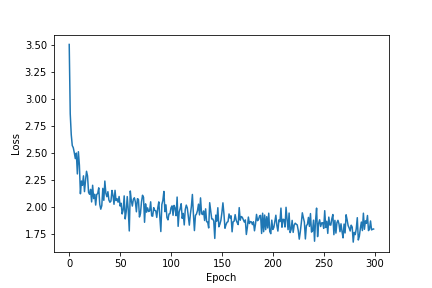
\includegraphics[scale=0.5]{simple_loss}
    \caption{RNN: SimplePoet Epoch vs. Loss}
    \label{fig:simplepoet}
    \end{center}
\end{figure}

The most sensible temperature appears to be 0.75 in Figure
\ref{fig:simple_temp075} although output is
quite a ways from being mistaken for a human. The most noticeable thing
about temperature is the amount of words that appear to be made up. When
temperature is too low or too high, the poem structure will appear to be in
place but the words seem made up.

\subsection{Improving RNNs}

Improvements to the SimplePoet RNN were based on Deep-speare
\cite{lau2018deepspeare} model. There appeared to be several good ideas
in this paper which could have been pursued in this assignment. I added
a fairly straight-forward feature from Deep-speare which included word
embeddings concatenated to character embeddings. The model took longer to
train but the example output, see Figure \ref{fig:fancy_temp075} appears
much more sensible than a strictly character based model. Quantitatively,
this model achieved a similar loss function to SimplePoet.

\begin{figure}
  \begin{center}
    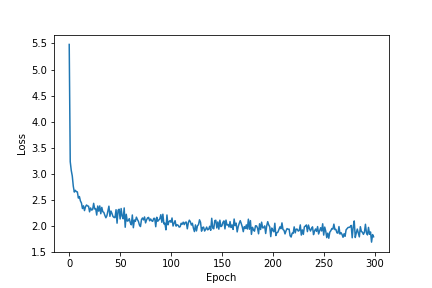
\includegraphics[scale=0.5]{fancy_loss}
    \caption{Improved RNN SimplePoet++ Epoch vs. Loss}
    \end{center}
  \end{figure}


\subsection{Discussion}

This assignment was helpful for
getting more familiar with RNN models. I was able to get qualitative
improvements with SimplePoet++ using word embeddings in addition to
character embeddings.Given more time, I would have liked to explore the
Deep-speare
\cite{lau2018deepspeare}  use of encoder/decoder models like the Seq2Seq
paper for generating Shakespeare Sonnets.


\bibliographystyle{unsrt}
\bibliography{references}


\subsection{Appendix}

\begin{figure}[h]
  \centering
  \begin{subfigure}[b]{\textwidth}
    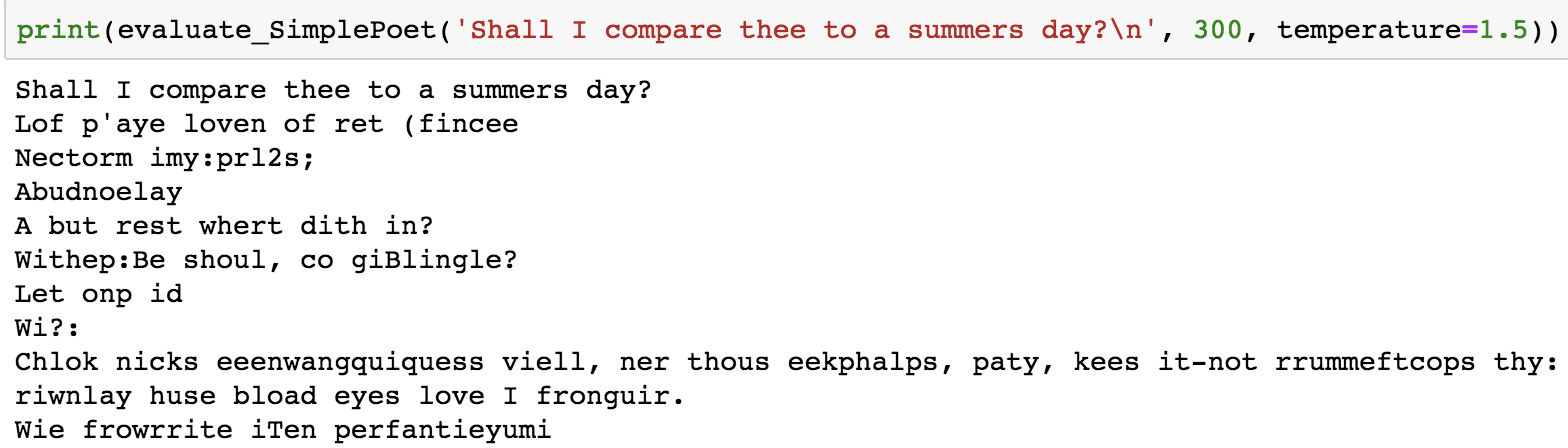
\includegraphics[width=\textwidth]{basic_temp15}
    \caption{SimplePoet, temperature=1.5}
    \label{fig:simple_temp15}
  \end{subfigure}

  % fig 2

    \begin{subfigure}[b]{\textwidth}
    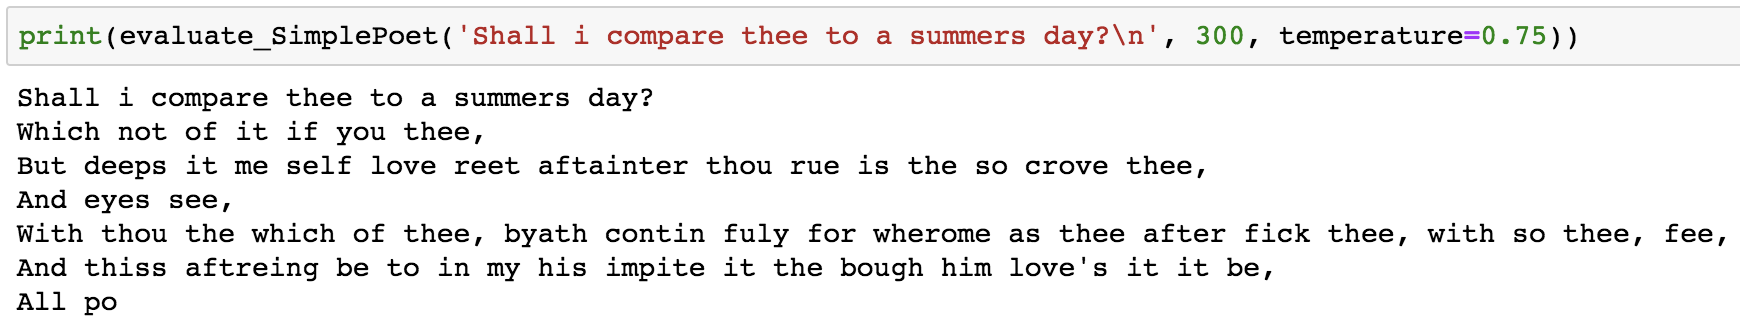
\includegraphics[width=\textwidth]{basic_temp075}
    \caption{SimplePoet, temperature=0.75}
    \label{fig:simple_temp075}
    \end{subfigure}

    % fig 3

      \begin{subfigure}[b]{\textwidth}
    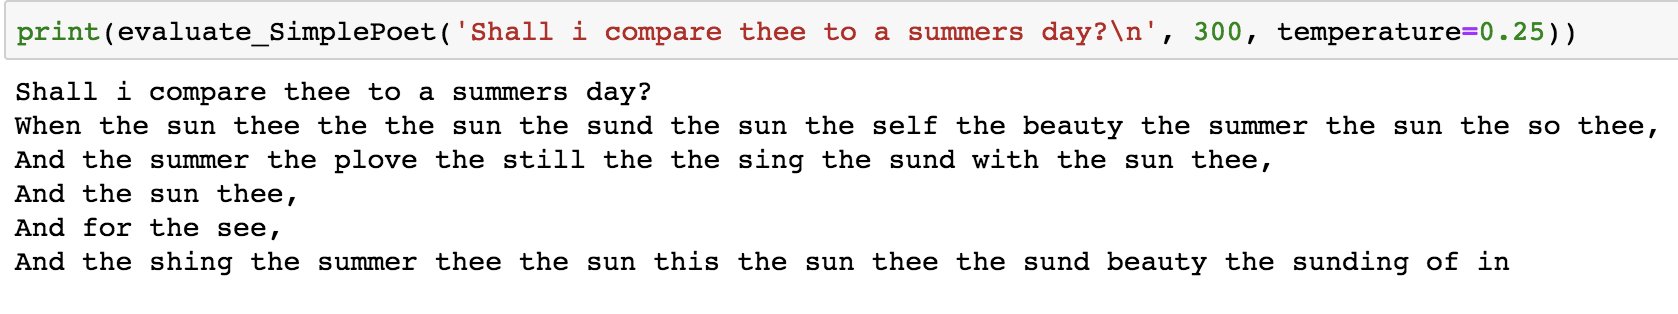
\includegraphics[width=\textwidth]{basic_temp025}
    \caption{SimplePoet, temperature=0.25}
    \label{fig:simple_temp025}
      \end{subfigure}

      % fig 4

        \begin{subfigure}[b]{\textwidth}
    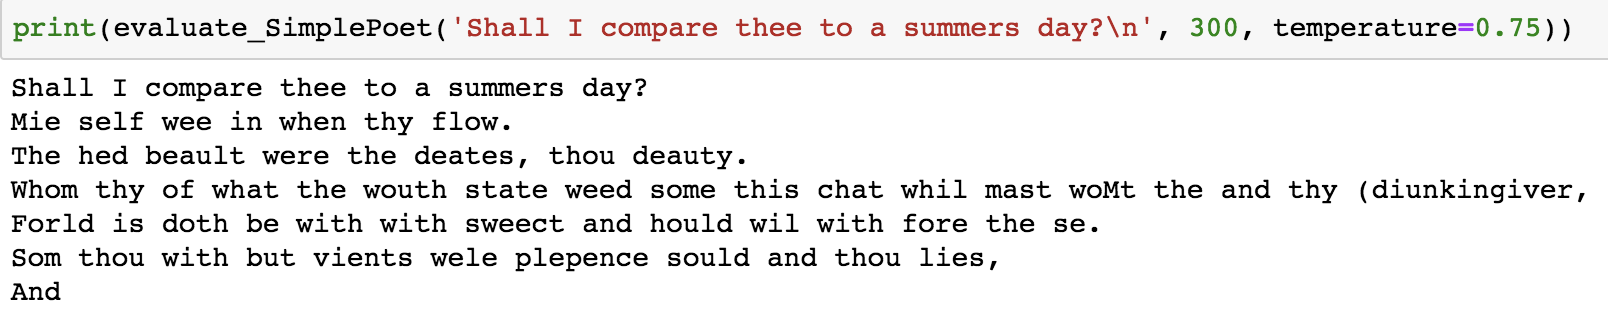
\includegraphics[width=\textwidth]{fancy_temp075}
    \caption{SimplePoet, added word embeddings, temperature=0.75}
    \label{fig:fancy_temp075}
        \end{subfigure}

        \caption{Poetry Output of RNN (SimplePoet) and Improved RNN
          (SimplePoet++)}
        \label{fig:poems}
\end{figure}


\end{document}
